\section{Topic Introduction}

\begin{frame}{Motivating Questions}
    \begin{columns}[T]
        \begin{column}{0.5\textwidth}
            \begin{enumerate}
                \item Do Large Language Models (LLMs) have intelligence?
                \item Are they taking over the software industry?
            \end{enumerate}
        \end{column}
        \begin{column}{0.5\textwidth}
            \begin{figure}[!htb]
                \centering
                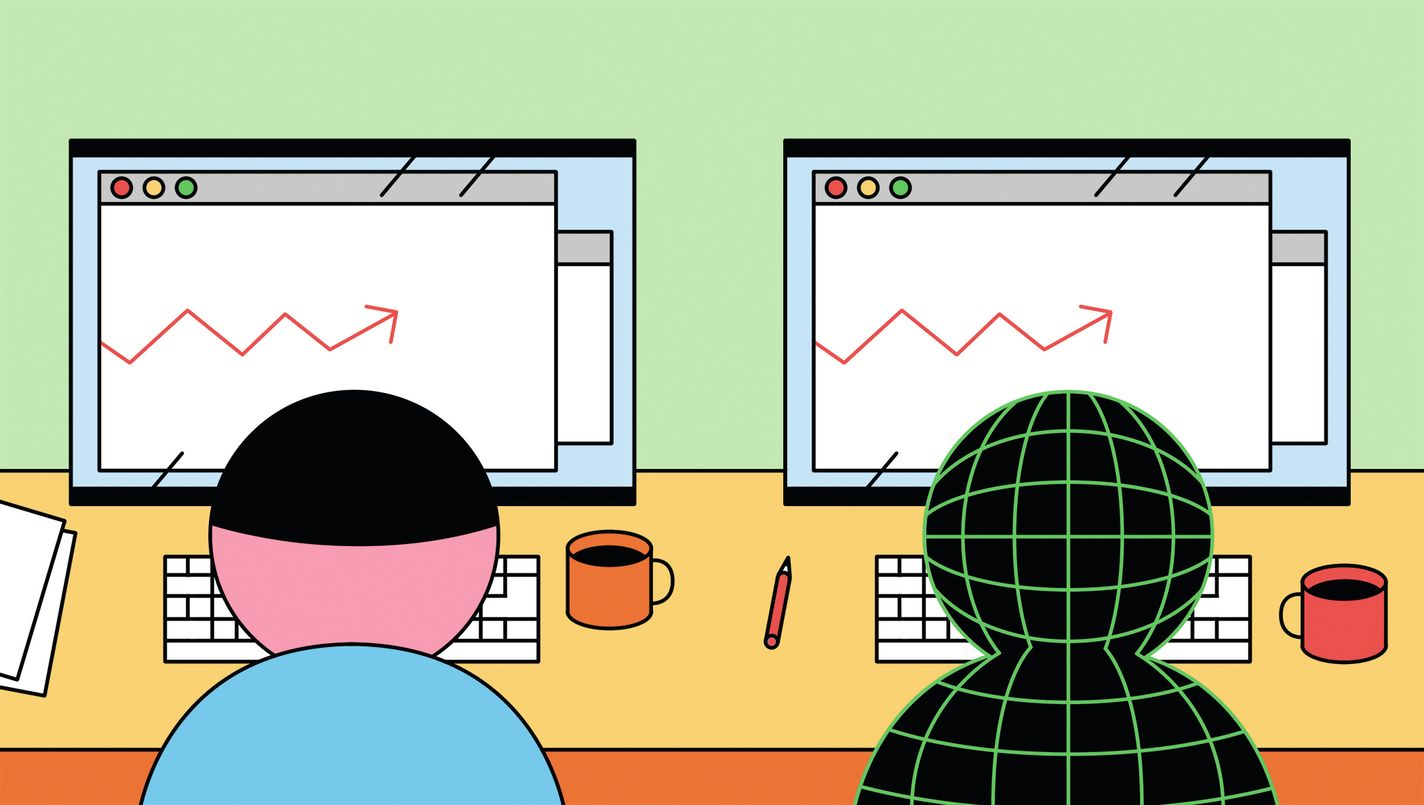
\includegraphics[scale=0.10]{img/ai_taking_jobs}
                \captionsetup{font=small}
                \caption{Your job is (probably) safe from artificial intelligence.\footnotemark[1]}
            \end{figure}
        \end{column}
    \end{columns}
    \footnotetext[1]{\footnotesize https://www.economist.com/finance-and-economics/2023/05/07/your-job-is-probably-safe-from-artificial-intelligence}
\end{frame}

\begin{frame}{Motivating Questions}
    By definition, intelligence is the ability to derive information, learn from experience, adapt to the environment, understand, and correctly utilize thought and reason~\cite{chollet2019measure}.\\
    \vspace{0.5cm}
    So what if we can create a machine that can do all of that?\\
    \vspace{1cm}
    \begin{figure}[!htb]
        \centering
        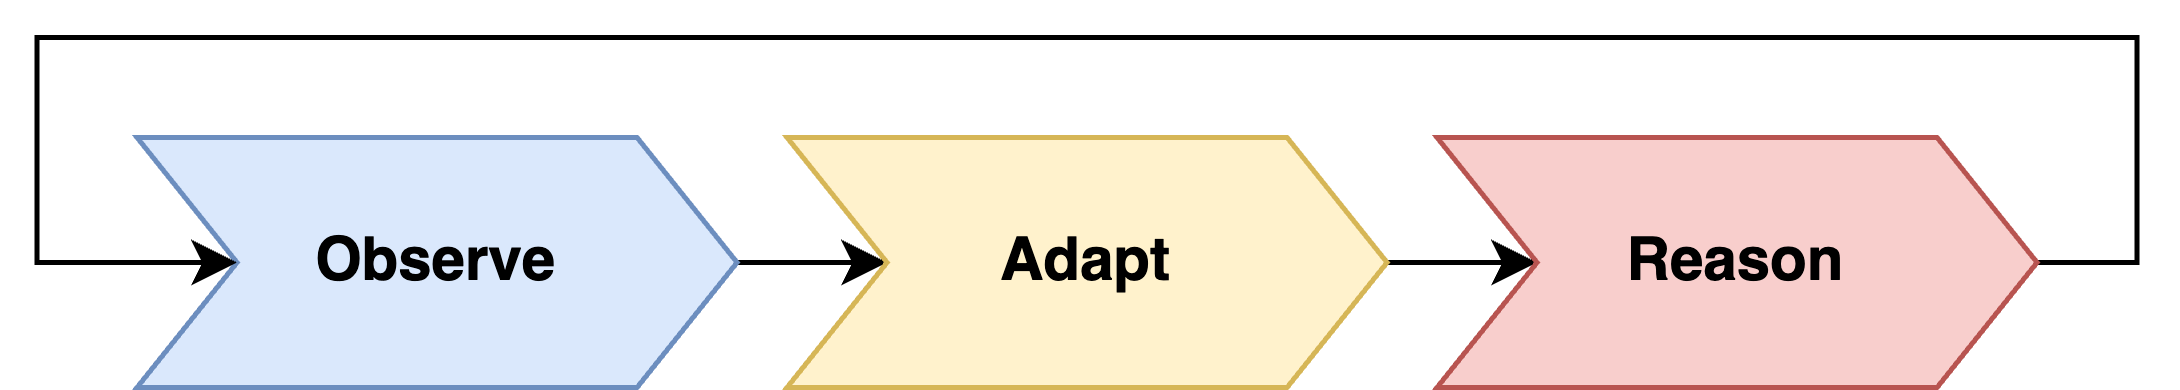
\includegraphics[scale=0.12]{img/intelligence}
        \captionsetup{font=small}
        \caption{Three components of intelligence.}
    \end{figure}
\end{frame}

\begin{frame}{Motivating Questions}
    \fontsize{14.4}{1}\selectfont A recent research from MIT concludes that AI-powered tools can help to reduce the completion time of software development tasks by 55.8\%~\cite{peng2023impact}.\\
    \vspace{1cm}
\end{frame}

\begin{frame}{Self-correcting LLMs}
    The objective of this research is to replicate the fundamental aspect of intelligence, specifically self-correction, in order to enhance the utility of LLMs in software development.\\
    \vspace{0.5cm}
    \begin{figure}[H]
        \centering
        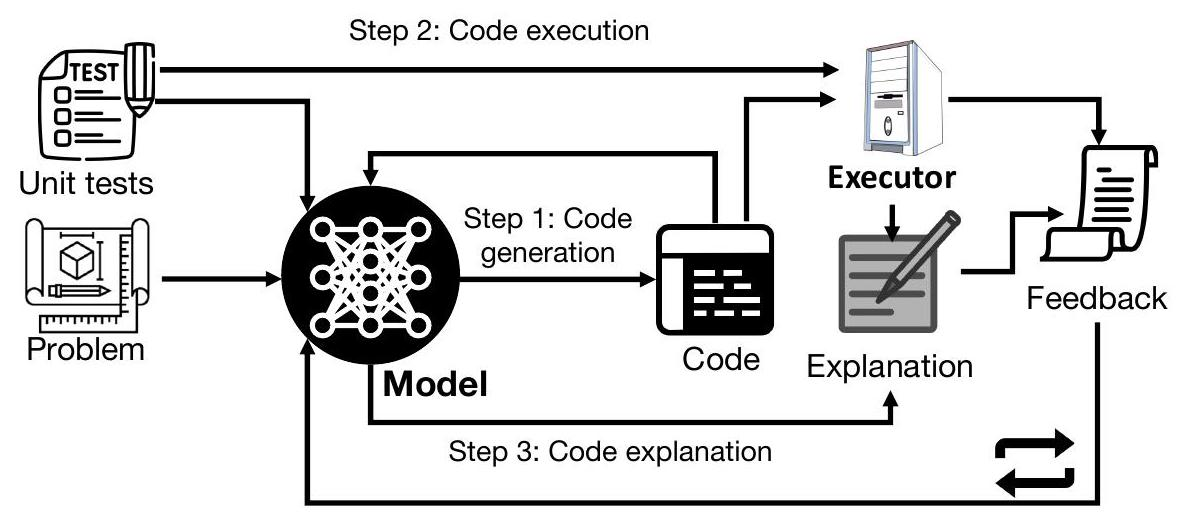
\includegraphics[scale=0.20]{img/self_debug}
        \caption{
            A prevalent approach for iterative debugging employing a large language model involves multiple steps~\cite{chen2023teaching}.}\label{fig:self_debug}
    \end{figure}
\end{frame}
